\documentclass[10pt,a4paper]{article}

\usepackage[utf8]{inputenc}
\usepackage[fleqn]{amsmath}
\usepackage{mathtools}
\usepackage{amsfonts}
\usepackage{amssymb}
\usepackage[alignedforall]{lpform}
\usepackage{enumitem}
\usepackage{graphicx}
\usepackage{float}
\usepackage{multicol}
\usepackage{lpform}
\usepackage{anziamjedraft}
%\usepackage{hyperref}


\begin{document}

\title{An interesting occurrence of a packing problem in Sports Jugger}
\author{C. Reeves}
\address{IBM Research Australia, 204 Lygon St Carlton, Victoria 305,3 \textsc{Australia}}
\email{claireelspeth@gmail.com}
\myorcid{0000-0002-7116-4657}
\date{\today}
\maketitle
\abstract{Sports Jugger is an amateur team sport growing in popularity across the globe. Participants in this sport make a lot of the equipment themselves; partly out of necessity, partly to reduce costs and partly because of a desire for customisation. We encountered an interesting version of a cutting stock or packing problem, which are well known mathematical optimisation problems, within this environment. When a Jugger club in Melbourne, Australia received a grant to obtain new equipment, the problem of achieving the greatest benefit to the club translated into a problem of cutting the optimal selection of pieces from a $2m\times1m$ foam block. 

In this paper we discuss the interesting aspects of this problem and present the heuristics used to develop the solution. This solution was successfully implemented and improved the previous best approach for cutting foam blocks to make Jugger sporting equipment. The implemented solution was able to construct two more items than the previous best approach, equivalent to a 15\% increase in items constructed per block, while also producing more useful spare pieces for storage. We also demonstrate that the solution found from heuristics is close to the optimal solution and is appealing to volunteers constructing equipment due to its simplicity.}
\section{Background}
In 2016, the Melbourne Jugger sporting club received a grant to purchase raw materials needed to make new equipment for the club. The grant provided sufficient funds to construct multiple teams worth of equipment at once by purchasing raw materials in bulk. However, equipment is constructed by volunteers who have previously not had large amounts of funding at once and usually make items one at a time. There has been little opportunity to minimise the wastage of bulk materials and optimise the usefulness of the complete set of items newly constructed.

This paper focuses on a single type of material used to create Sports Jugger equipment - foam padding - and uses mathematical optimisation to maximise utility of a block of foam. The club used foam blocks that cost \$120 for a single $2m \times 1m$ block of foam with a depth of $3cm$. Achieving the best use for each individual block of foam allows the club to make more equipment from the same amount of funding.

There are two related types of problems, well known in mathematical optimisation, that can be applied to this problems of this nature. Cutting stock problems minimise the length of a fixed width resource that is required to cut a specific number of items while packing problems maximise the utility of items which can fit inside a resource with fixed capacity. There is a large amount of literature on both types of problems. 

However, the specifics of the problem described in this paper are unusual and make it an interesting problem from a mathematical perspective. Multiple pieces of foam, sometimes of different sizes, are required to make a single item of equipment. Leftover pieces can be stored but are not as useful as pieces used immediately. Duplicate items of equipment are allowed to have a different utility and the number of each item to make is not fixed. Therefore, the problem of interest is similar to a packing problems with an additional assignment component to determine which items to make using the pieces cut from the foam block. For the remainder of this paper, we use the word item to describe a completed item of equipment that requires multiple pieces of foam.

In the rest of this paper we outline the specifications of items to be constructed for the Sports Jugger Problem in Section \ref{section:sparspecs}, review the literature on two dimensional cutting and packing problems in Section \ref{section:litreview}, describe the heuristics used to find the implented solution in Section \ref{section:heuristics}, present a mathematical model to find an optimal solution in Section \ref{section:mathmodel} and finally discuss the quality of our solution in Section \ref{section:results}.

\subsection{Problem Specifications}
There are several items of equipment, or combinations of equipment, that may be used by players on a Sports Jugger team. Full specifications and the usages of each item are available on the website for the Australian Jugger League Inc \cite{AJLweb}. The items which require pieces to be cut from the foam blocks are shown in Figure \ref{fig:spartypes} with the foam padding requirements presented in Table \ref{tab:sparpieces}. All of these use cylinders of $6cm$ diameter of varying lengths. A single cylinder is constructed from two pieces cut from the foam block. Cut pieces have dimensions equal to \textit{desired length} $\times$ $6cm$ \textit{width} $\times$ $3cm$ \textit{depth}. Two pieces of equal length are then glued together around a core and the corners trimmed to create a `roughly cylindrical' octagon. 

\begin{figure}
\centering
\includegraphics[scale=0.5]{SparSpecs.png} 
\caption{Equipment used in Sports Jugger. Image courtesy of the Australian Jugger League Inc.}
\label{fig:spartypes}
\end{figure}

\begin{table}
\centering
\begin{tabular}{l|l}\hline
Q-tip & $2 \times 60cm$ cylinders\\
Staff & $1 \times 100cm$ cylinder $+ 1 \times 50cm$ cylinder\\
Long & $ 1 \times 100cm$ cylinder\\
Short & $1 \times 75cm$ cylinder\\\hline
\end{tabular}
\caption{Maximum size of the foam pieces required to construct specific items of equipment for Sports Jugger}
\label{tab:sparpieces}
\end{table}

\label{section:sparspecs}

It is desirable for players to have access to a variety of equipment as well as a sufficient quantity of equipment. The problem needs to allow the utility of duplicate items to decrease and should also allow for different utility values of individual items to represent the popularity of certain items over others. 

Items also require multiple pieces and may be competing with other item types in order to receive those pieces. This requires the problem to not only determine how many pieces to cut from the block of foam but to also assign pieces to each item. Furthermore, the rules for Jugger in Australia also allow for flexible padding section lengths. In other words, there is both a minimum and a maximum length of padding specified for each item and items may use either of these limits or any length in between. This increases the number of potential cutting patterns drastically. For this problem, it is assumed that all items are to be made with the maximum length of the padding section. This reduces the problem to a much more manageable size and still allows customisation of items of shorter lengths if desired after the pieces are cut.

There are still a large number of potential cutting patterns in this problem. There may be between 33 and 66 pieces cut from a single block and pieces may be cut from the block in two different directions (i.e. at $0^{\circ}$ or $90^{\circ}$).  The problem presented is complex. It is a 2D integrated problem requiring both piece packing and assignment, made more interesting as value of each completed item reduces as the number of duplicates increases and the large number of possible patterns.

\subsection{Cutting and Packing Problems}

In this section, we briefly review the literature on cutting and packing problems in two dimensions. The packing part of the Sports Jugger equipment problem involves packing rectangular pieces into a larger rectangle to generate cutting patterns. We therefore concentrate the review on rectangular cutting stock problems and knapsack problems.  These are classical NP hard problems and, as such, there are no known algorithms to find optimal solutions in polynomial time \cite{Kenyon2000} \cite{Leung2012}. 

There are many real world examples of cutting stock problems. These problems commonly minimise the length of a resource used to fulfil a requested order.  Reviews of cutting stock problems include descriptions of sub-classes of the cutting stock problem, such as bin packing and strip packing problems, as well as discussing solution approaches \cite{haessler1991} \cite{Lodi2002} \cite{Cheng}. A related class of problem also discussed in \cite{Cheng} is the assortment problem. This optimises the size of stock resources to have on hand. This is relevant to many cutting stock problems as the average percentage wastage in a two dimensional problem depends on the characteristics of the resources available.

Two-dimensional cutting stock problems are more complex than one dimensional problems even when limited to rectangular shaped pieces only. This is due to the the necessity to define and generate feasible cutting patterns. Gilmore and Gomory \cite{GilmoreGomory} solve a two dimensional problem using a two stage approach. The problem itself involves a stock rectangle of a given width and length and a set of smaller demand rectangles of varying width and length. The objective is to minimise the number of stock rectangles used. With a two stage solution approach, rectangular resources are first cut into strips using parallel cuts. These strips are then further divided using perpendicular cuts. Solving the model frequently involves optimising how many times each feasible cutting pattern appears in the solution, using a column generation approach to add or remove different feasible cutting patterns. The difficulty in solving the model is in the number of feasible cutting patterns that exist. Generation of patterns is approached by solving a generalised knapsack problem with dynamic programming \cite{GilmoreGomory} \cite{haessler1991} \cite{Cintra2008}. Over time, these solution approaches have been improved by methods such as limiting the number of times pieces of a given size can appear in cutting patterns \cite{haessler1991}. 

Kenyon and R\'{e}mila \cite{Kenyon2000} address a problem where a rectangle of fixed width and sufficiently large height is available. They seek near optimal solutions, using an approximation algorithm, to the problem of packing $n$ smaller rectangles into the larger rectangle in a pattern that minimises the total height used to fit the $n$ rectangles. They do not allow rotation of rectangles. The solution approach presented is an approximation algorithm for determining a cutting pattern. They develop configurations that select out a subset of rectangles whose combined width is less than the width of the enveloping rectangle. Horizontal strips at different heights are then associated with configurations. The total height is minimised by minimising the number of strips required to fit all pieces.

Schutt, Stuckey and Verden \cite{schutt2011} present a paper on optimal carpet cutting. Like many other problems, they require a given set of pieces to be cut from a resource and seek to minimise the length of resource required. The carpet cutting problem allows for many different shapes and sizes and permits some rotation of pieces. They use constraint programming techniques to ensure that pieces do not overlap and symmetry breaking to improve the capability of the model to prove optimal solutions. As a result, they increase the number of solutions to typical problems proven to be optimal when compared to existing methods which find, but do not prove, optimal solutions.

The knapsack problem maximises the value of items packed into a single object with limitations capacity such as weight or volume. It has also been used in the literature to generate cutting patterns which may be used in a two stage cutting stock problem \cite{GilmoreGomory}. However, the Sports Jugger problem has diminishing returns on packing multiple items. This then affects the value of cutting additional pieces of the same length, which could be assigned to multiple items of the same type or a different type of item altogether, thus increasing the complexity of our problem. The unbounded knapsack problem allows multiple copies of the same piece to be packed into a single resource \cite{Kellerer2004} but does not consider the aspect of diminishing return on value.

Maximising the value of a non-monotonic function, subject to knapsack contraints, has been discussed as a generalised problem. For this type of problem, it is possible to provide approximation algorithms \cite{jonlee2009}. Approximation algorithms are solution approaches to NP hard problems which guarantee that the quality of a result found in polynomial time will be no more, or no less for a maximisation problem, than the optimal solution multiplied by a proven factor. 

Two dimensional knapsack problems are also present in the literature alongside heuristic solution approaches for these problems \cite{Egeblad2009} \cite{Leung2012}. Rectangles are packed into larger stock objects and rotation of rectangles may be allowed \cite{Egeblad2009}. Decision variables specify whether a rectangle is packed while constraints limit the coordinates of each rectangle. A Simulated Annealing metaheuristic is used to add or remove rectangles and this approach can also be implemented for three dimensional problems \cite{Egeblad2009}. Simulated Annealing can also be hybridised with a constructive heuristic for the rectangle knapsack packing problem \cite{Leung2012}.

There is a vast amount of literature on cutting and packing problems \cite{SweeneyRidenour} and yet it is still a relevant field of research due to the broad area of application and difficulty in proving optimal solutions. The problem arising from the need to construct equipment for Sports Jugger is a packing problem where total resource area is fixed and there is flexibility in choosing which rectangular pieces to cut. These pieces may also be rotated and that increases the number of feasible cutting patterns. This type of problem, that of a two dimensional knapsack problem, is present in the literature and can be solved with metaheuristics \cite{Egeblad2009}. Approximation algorithms can provide solutions to problems with knapsack constraints, even when there is a diminishing return on value present in the maximisation function, and guarantee a particular solution quality \cite{jonlee2009}. However, the problem we encounter here also states that pieces must be assigned to items and have little individual value.  Our literature search to date has not identified any models containing packing, assignment and diminishing returns in a single problem.

\label{section:litreview}
\section{Heuristic Solution Approach}
\label{section:heuristics}
The solution to the problem was developed in close consultation with the volunteers who would be measuring and making the cuts. They specified a strong desire for a simple solution and needed a solution quickly. Materials had already been purchased and completed items were required for an upcoming Sports Jugger tournament. Speed and simplicity influenced our choice to use a basic heuristic solution approach.

Additional assumptions were introduced to simplify the problem further. We continue to use the assumption that pieces will always be cut exactly to their maximum length. The next assumption is that only guillotine cuts can be made. A guillotine cut is a straight cut that goes from one edge of a section all the way through to the opposing edge. This is a type of cut common to many cutting stock problems and results in patterns much easier to measure and cut. We also assume that pieces of the same type will be cut from the same subsection of the foam block dedicated to that type of piece. These subsections must contain at least a minimum number of pieces of the same type that is greater than one and should contain the full complement of required pieces of the same type where possible. It is allowable to have multiple subsections dedicated to the same type of piece but the area of each of these subsections must be large enough to contain multiple copies of the same piece. This assumption was introduced allow volunteers to cut a block into sections that are then distributed to different people tasked with cutting multiple copies of the same piece. This is a reasonable assumption to make because there will be no wastage of foam between pieces of the same size, however, there is still the possibility of wasted foam between sections.

Next, capacity planning was undertaken. This determined a pool of solutions that would be acceptable to the club and did not exceed the total area of the foam block. This creates a minimal order quantity and a maximal order quantity of each piece but there is some residual flexibility for the optimal order.

We began by exploring the basic set of equipment that was needed to outfit two Sports Jugger teams. This included one of each type of item per team, with the exception of Short Spars where two were required per team, and resulted in 62.4\% of the foam blocks total area being utilised. In consultation with the club, we then added in extra items into the pool in order of perceived utility until close to 100\% of the total area of the foam block would be used to make the set of items. This was repeated to get a pool of solutions with similar utility. Results from this process returned the maximum number of each type of item to make and hence indicated how many pieces of each length we should try to fit into a cutting pattern. These quantities are displayed in Table \ref{tab:caplan}. We also display the width the would be required to fit the number of pieces specified.  

\begin{table}
\centering
\begin{tabular}{l|ll}\hline
\textit{Item Type} & QTY&\\
Q-tip & 3--4&\\
Staff & 3--4&\\
Long & 3--5&\\
Short & 4--6&\\\hline
\textit{Piece Length} & QTY& Width\\
100cm & 12--16& 72--96cm\\
75cm & 8--12 & 48--72cm\\
60cm & 12--16 & 72--96cm\\
50cm & 6--8& 36--48cm\\\hline
\end{tabular}
\caption{Bounds on the quantity of each item type that will fit in good solutions and corresponding quantity of each piece length and total width required to cut that quantity of pieces.}
\label{tab:caplan}
\end{table}

The use of Table \ref{tab:caplan} is limited as it is not possible to construct the maximum quantity of each item type from a single block of foam. It is instead intended to help guide the application of the heuristics. The heuristic approach uses a \textit{Greatest Need First} approach.  This is different to classical heuristic strategies such as \textit{Next-Fit Decreasing Height}, \textit{First-Fit Decreasing Height} or \textit{Best-Fit Decreasing Height} which position pieces in levels and use height to determine the next piece to select.
 
Basic rules determine where to make cuts and to determine in which direction each piece length should be cut. 

\begin{enumerate}
\item Assign priority to pieces based on number required
\item Position cuts where at least one side of each resulting section is compatible with the length of priority pieces
\item Assign priority pieces to sections
\item Subdivide newly assigned section such that
\begin{enumerate} \item one section has a width within the desired width range for the assigned piece length, and\item the other section  has at least one side compatible with a different piece length (where possible)
\end{enumerate}
\item Assign the appropriate piece length to the subdivided section
\item If any piece lengths are assigned a total area greater than required
\begin{enumerate}
\item Unassign all areas assigned to that piece length (but maintain any subdivision of sections)
\item Reduce the priority of that piece length
\end{enumerate}
\item Repeat steps 2 to 6 until no more subdivisions can be made
\end{enumerate}

\begin{figure}
\centering
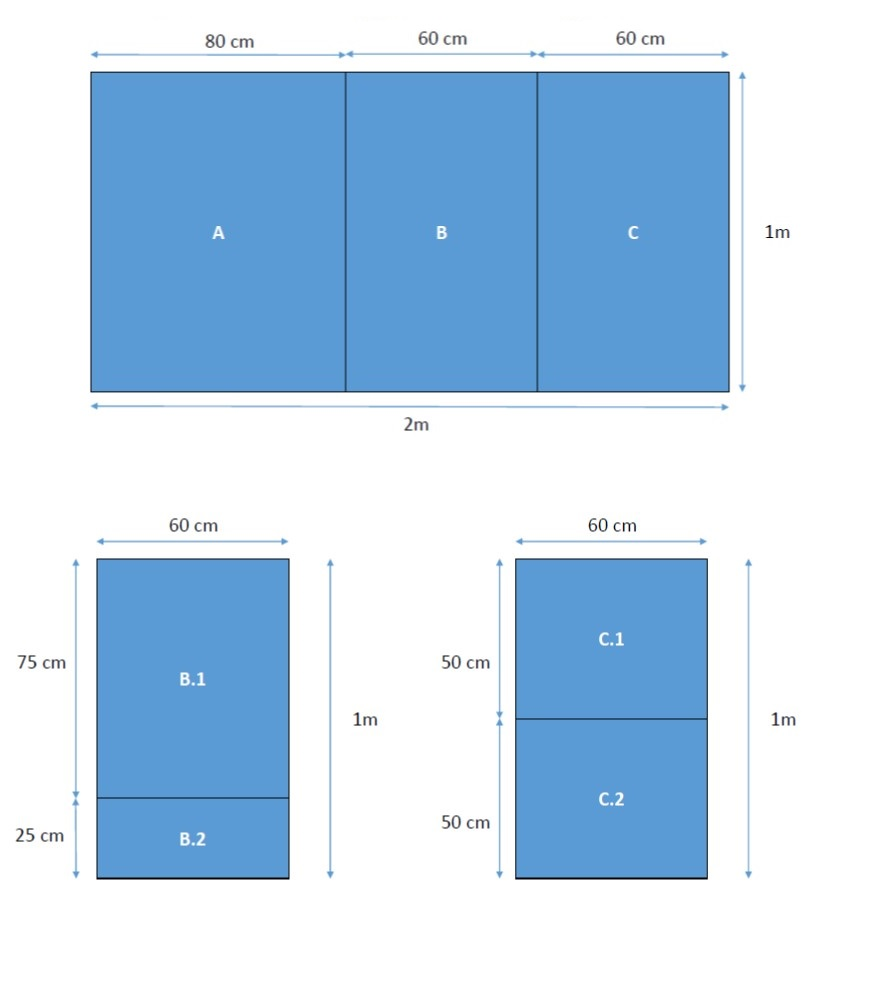
\includegraphics[scale=0.5]{FoamCutting/sectionsAll.jpg} 
\caption{Solution to the cutting problem using the heuristic approach. Area A is dedicated to cutting $100cm$ lengths, area B.1 is dedicated to cutting $75cm$ lengths, area C.1 is dedicated to cutting $50cm$ length and both area B.2 and C.2 are dedicated to cutting $60cm$ lengths.}
\label{fig:heursol}
\end{figure}

Applying these rules led to the solution depicted in Figure \ref{fig:heursol}. In this solution, $100cm$, $75cm$, and $50cm$ lengths are all cut in the same direction, relative to the original dimensions of the foam block, in their assigned sections while $60cm$ lengths are cut at a $90^{\circ}$ rotation in two sections. A detailed description of the development of this solution is described here.
\begin{enumerate}
\item Assign priority to $100cm$ and $60cm$ lengths
\item Make a cut returning sections with dimensions $60cm \times 100cm$ (Section C) and $140cm \times 100cm$ (Section AB)
\item Assign $60cm\rightarrow$ C, $100cm\rightarrow$ AB
\item Cannot subdivide C
\item Subdivide AB with a cut returning $80cm \times 100cm$ (Section A) and $60cm \times 100cm$ (Section B) 
\item Assign $100cm\rightarrow$ A, $60cm\rightarrow$ B
\item $60cm$ lengths are over assigned, reduce priority and unassign B and C
\item Assign priority to $75cm$ lengths
\item Make a cut dividing section B into $60cm \times 75cm$ (Section B.1) and $60cm \times 25cm$ (Section B.2)
\item Assign $75cm\rightarrow$ B.1, $60cm\rightarrow$ B.2
\item Assign priority to $50cm$ lengths
\item Make a cut dividing section C into $60cm \times 50cm$ (Section C.1) and $60cm \times 50cm$ (Section C.2)
\item Assign $50cm\rightarrow$ C.1, $60cm\rightarrow$ C.2
\item Done
\end{enumerate}

These heuristic rules are able to be applied without any specialised software. Once pieces are cut, they are assigned to item types in order of utility. The quality of this solution is discussed in Section \ref{section:results}. 

\section{Exact Solution Approach}
It is also possible to represent the packing and assignment problem for Sports Jugger using mathematical modelling techniques. An integrated Mixed Integer Programming model is formulated that contains decision variables specifying the location and orientation of each piece that will be cut from the foam block and assigns cut pieces to items that will be made. Disjunctive constraints are used to ensure that pieces do not overlap.
We implemented the model in ILOG CPLEX Optimization Studios 12.2, running on an Intel i5-4300U CPU and returned solutions and optimality gaps at different time limits. 

\label{section:mathmodel}
\subsection*{Sets \& Parameters}
\begin{itemize}
\item[$F_x=$] \textit{200cm}, $x-$dimension of the foam block
\item[$F_y=$] \textit{100cm}, $y-$dimension of the foam block
\item[$E=$] \{\textit{Q-tip, Long, Staff, Short}\}, Equipment
\item[$L=$] \{\textit{100cm, 75cm, 60cm, 50cm}\}, Piece lengths
\item[$P$] Set of all pieces
\item[$\ell_p$] Length of piece $p$
\item[$w= $] \textit{6cm}, Width of all pieces
%\item[$P^{100}$] Set of all pieces with length \textit{100cm}
%\item[$P^{75}$] Set of all pieces with length \textit{75cm}
%\item[$P^{60}$] Set of all pieces with length \textit{60cm}
%\item[$P^{50}$] Set of all pieces with length \textit{50cm}
\item[$U_e =$] [4,5,4,6], Upper bound on the number of items of each equipment type to make
\item[$O^e=$] $1..U_e$, Ordered set of individual items to make for each equipment type $e$
\item[$B_{oe}$] [[1,1,0.5, 0.25],[1,1,0.5, 0.33, 0.25], [1,1,0.5, 0.33],[1,1,0.75, 0.75,0.5,0.25]] Benefit of completing each item for each equipment type
\item[$N_{le} = $] [[0,0,4,0],[2,0,0,0], [2,0,0,2],[0,2,0,0]] Number of pieces of each length $l$ required to complete an item of equipment $e$
\item[$M=$] 1000, A large value for logical constraints
\item[$\epsilon=$] 0.001, A small weighting value for a secondary objective concerning the utility of leftover pieces
\end{itemize}
The $x$ and $y$ coordinates are defined such that the origin is the bottom left corner of the foam block. Thus, larger $x$ values move towards the right and larger $y$ values move upwards.
\subsection*{Decision Variables}
%\begin{tabular}{p{0.5cm}p{9cm}}
%$x_p $& $x-$position where piece $p\in P$ begins (i.e. left-most position on the foam block where piece $p\in P$ is present)\\
%$y_p$& $y-$position where piece $p$ begins (i.e. top-most position on the foam block where piece $p$ is present)\end{tabular}
%\begin{eqnarray*}
%r_{p} &=& \begin{cases}
%			1 & \begin{split}\text{if piece $p$ is rotated to have the long}\\\text{ side cut parallel to the $x-$axis,}\end{split}\\
%			0 & \begin{split}\text{if piece $p$ is not rotated and has the}\\\text{ long side cut parallel to the $y-$axis,}\end{split}
%		\end{cases}\\
%			z_{p} &=& \begin{cases}
%			1 & \begin{split}\text{if piece $p$ cut from the foam block,}\end{split}\\
%			0 & \text{otherwise}
%		\end{cases}\\
%		u_{pq} &=& \begin{cases}
%			1 & \begin{split}\text{if piece $q\in P$ is to the right of piece $p\in P$,}\end{split}\\
%			0 & \text{otherwise}
%		\end{cases}\\
%		v_{pq} &=& \begin{cases}
%			1 & \begin{split}\text{if piece $q\in P$ is below piece $p\in P$,}\end{split}\\
%			0 & \text{otherwise}
%		\end{cases}\\
%		w^x_{pq} &=& \begin{cases}
%			1 & \begin{split}\text{if piece $q\in P$, to the right of piece $p \in P$,}\\\text{ overlaps with piece $p$ in the $x-$plane,}\end{split}\\
%			0 & \text{otherwise}
%		\end{cases}\\
%		w^y_{pq} &=& \begin{cases}
%			1 & \begin{split}\text{if piece $q\in P$, positioned below piece $p \in P$,}\\\text{ overlaps with piece $p$ in the $y-$plane,}\end{split}\\
%			0 & \text{otherwise}
%		\end{cases}\\
%				c_{oe}& =& \begin{cases}
%			1 & \begin{split}\text{if $o^{th}$ item of equipment type $e$ is complete}\end{split}\\
%			0 & \text{otherwise}
%		\end{cases}
%		\end{eqnarray*}
%		\begin{tabular}{p{0.5cm}p{11cm}}
%$a_{le}$ & number of pieces of length $l \in L$ assigned to equipment type $e \in E$%\\
%\end{tabular}
%
\begin{tabular}{p{0.5cm}p{9cm}}
		$x_p $& $x-$position where piece $p\in P$ begins (i.e. left-most position on the foam block where piece $p\in P$ is present)\\
$y_p$& $y-$position where piece $p$ begins (i.e. lower-most position on the foam block where piece $p$ is present)\\\\
$r_{p}=$ & $
\left\lbrace \begin{aligned}1 & \text{\ \ if piece $p$ is rotated to have the long side} \\& \text{\ \ cut parallel to the $x-$axis,}&\\
0 &\text{\ \ if piece $p$ is rotated to have the long side} \\& \text{\ \ cut parallel to the $y-$axis,}&\\
\end{aligned} \right.
$\\\\

$t_{p} =$& $
\left\lbrace \begin{aligned}
			1 & \text{\ \ if piece $p$ cut from the foam block,}&\\
			0 & \text{\ \ otherwise}&\\\end{aligned} \right.$\\\\
			
			
			$u_{pq} =$& $
\left\lbrace \begin{aligned}
			1 & \text{\ \ if piece $q\in P$ is to the right of piece $p\in P$,}&\\
			0 & \text{\ \ otherwise}&\\\end{aligned} \right.$\\\\
			
			$v_{pq} =$& $
\left\lbrace \begin{aligned}
			1 & \text{\ \ if piece $q\in P$ is above piece $p\in P$,}&\\
			0 & \text{\ \ otherwise}&\\\end{aligned} \right.$\\\\			
		
		
				$z_{pq} =$& $
\left\lbrace \begin{aligned}
			1 & \text{\ \ if piece $q\in P$, to the right of piece $p \in P$,} \\&
			\text{\ \ overlaps with piece $p$ in the $x-$plane,}&\\
			0 & \text{\ \ otherwise}&\\\end{aligned} \right.$\\\\	
		
%					$w^y_{pq} =$& $
%\left\lbrace \begin{aligned}
%			1 & \text{\ \ if piece $q\in P$, positioned below piece $p %\in P$,} \\&
%			\text{\ \ overlaps with piece $p$ in the $y-$plane,}&\\
	%		0 & \text{\ \ otherwise}&\\\end{aligned} \right.$\\\\	
	
		
			$c_{oe} =$& $
\left\lbrace \begin{aligned}
			1 & \text{\ \ if $o^{th}$ item of equipment type $e$ is complete,} &\\
			0 & \text{\ \ otherwise}&\\\end{aligned} \right.$\\\\	
			
$a_{le}$ & number of pieces of length $l \in L$ assigned to equipment type $e \in E$\\

\end{tabular}

				
\subsection*{Mixed Integer Programming Model}
In this model we maximise the benefit returned from all completed orders (1). 

A second term is also introduced to maximise the utility of leftover pieces for future use. Here, we sum all of the pieces cut from the foam block and then subtract all of those assigned to completed items. This returns the number of unassigned pieces left over. 

Storing leftover pieces is less useful than completing items immediately, however, a solution that returns storable pieces for later use should outperform a solution that completes the same set of items but wastes the rest of the foam. As larger pieces can trimmed down to smaller sizes, and are thus more flexible and valuable, we also scale this term by the size of the spare pieces. This requires a coefficient (i.e. $\epsilon$) able to convert the length of spare pieces in $cm$ into a utility value. The value should also consider that the utility of spare pieces should be smaller than the utility of completed items.

\begin{lpformulation}
\lpobj{max}{\sum_{e \in E}\sum_{o \in O^e}c_{oe} B_{oe} + \epsilon\left(\sum_{p \in P}t_p\ell_p - \sum_{l \in L}\sum_{e \in E}a_{le}l\right)}
\end{lpformulation}


%The maximisation function is then subject to a set of constraints.

\begin{lpformulation}
\lpeq{\sum_{o \in O^e} c_{oe}\times N_{le} \leq a_{le}}{e \in E, l \in L}
\lpeq{\sum_{e \in E} a_{le}\leq \sum_{p \in P: \ell_p = l}t_p}{l \in L}
\end{lpformulation}


An ordered item is considered complete \textit{iff} it is assigned all of the cut pieces that it requires. Constraint (2) ensures that each completed item has sufficient pieces assigned while Constraint (3) limits the number of pieces assigned to the number of pieces actually cut.

Pieces may only be cut within the physical boundaries of the foam block. Constraints (4) and (5) ensure each piece begins within the block. Constraints (6) and (7) make sure that pieces do not extend beyond the edges of the block.

\begin{lpformulation}
\lpeq{0\leq x_p\leq F_x}{p \in P}
\lpeq{0\leq y_p\leq F_y}{p \in P}
\lpeq{F_x-x_p -\ell_p\left(1-r_p\right)-wr_p \geq 0}{p \in P, e \in E}
\lpeq{F_y-y_p -w\left(1-r_p\right)-\ell_p r_p \geq 0}{p \in P, e \in E}
\end{lpformulation}

Pieces which are cut from the foam block may share boundaries but not occupy the same physical space on the foam block. Disjunctive constraints are introduced to enforce that if pieces overlap with each other in one dimension then they cannot overlap in the other dimension. In order to establish these constraints, we must first identify the relative position of pieces to each other.

Constraint (8) sets the variable $u_{pq} = 1$ if piece $q$ has the same or a larger $x-$position than piece$p$.  
\begin{lpformulation}
\lpeq{M u_{pq}\geq x_q-x_p}{p,q \in P: p\neq q}
\end{lpformulation}

Constraint (9) similarly sets the variable $v_{pq} = 1$ if piece $q$ has the same or a larger $y-$position than piece$p$.
\begin{lpformulation}
\lpeq{M v_{pq}\geq y_q-y_p}{p,q \in P: p\neq q}
\end{lpformulation}

If two pieces have the same starting position in either the $x-$ or $y-$ dimension, then the piece with the larger index will be considered to be placed to the right or above the other. Constraints (10) and (11) apply this rule in the $x-$ and $y-$ dimensions respectively.
\begin{lpformulation}
\lpeq{M u_{pq}\geq x_q-x_p +1}{p,q \in P: p< q}
\end{lpformulation}
\begin{lpformulation}
\lpeq{M v_{pq}\geq y_q-y_p +1}{p,q \in P: p< q}
\end{lpformulation}

Constraint (12) then introduces a disjunctive variable that tracks whether one piece overlaps with another piece in the $x-$dimension.  We use logical constraints so that piece $q$ will only be counted as overlapping with a different piece $p$ if certain conditions are met. These conditions are that: both pieces $p$ and $q$ must be cut from the foam block, piece $q$ must be positioned to the right of piece $p$, and the $x-$position of piece $q$ falls within the $x-$range where piece $p$ will be cut. 

\begin{lpformulation}
\lpeq{M\left(z_{pq} + 3 - t_p- t_q - u_{pq}\right)\lpnewline\geq x_p - x_q -\ell_p\left(1-r_p\right)+wr_p}{ p,q \in P: q\neq p}
\end{lpformulation}

If two pieces $p$ and $q$ are overlapping in the $x-$ dimension then the variable $z_{pq}$ will equal $1$. When this occurs, Constraints (13) and (14) prevent the same two pieces overlapping in the $y-$dimension. Constraint (13) prevents pieces $p$ and $q$ from overlapping in the case where piece $q$ is positioned above piece $p$. Constraint (14) is similar but applies when piece $p$ is positioned above piece $q$.


\begin{lpformulation}
\lpeq{M\left(z_{pq} + 3 - t_p- t_q - v_{pq}\right)\lpnewline\geq y_p - y_q -w\left(1-r_p\right)+\ell_p r_p}{p,q \in P: q\neq p}
\lpeq{M\left(z_{pq} + 3 - t_p- t_q - v_{qp}\right)\lpnewline\geq y_q - y_p -w\left(1-r_q\right)+\ell_q r_q}{p,q \in P: q\neq p}
\end{lpformulation}



%Constraint (13) applies the same logic for pieces potentially overlapping in the $y-$dimension. For both Constraint (12) and Constraint (13), we use logical constraints so that piece $q$ will only be counted as overlapping with a different piece $p$ if certain conditions are met. These conditions are that: both pieces $p$ and $q$ must be cut from the foam block, piece $q$ must be positioned to the right of, or below, piece $p$, and the position of piece $q$ falls within the range where piece $p$ will be cut.
%
%\begin{lpformulation}
%\lpeq{M\left(w^y_{pq} + 3 - t_p- t_q  - v_{pq}\right)\lpnewline\geq y_p - y_q -w\left(1-r_p\right)+\ell_p r_p}{p,q \in P: q\neq p}
%\end{lpformulation}
%
%In Constraints (15) and (16), we specify that if pieces $p$ and $q$ can only overlap in either the $x-$plane or the $y-$plane but not both. We require two constraints to make sure that when a piece to the right of another piece has been identified as overlapping, we then prevent overlapping of those two piece regardless of which is below the other.
%\begin{lpformulation}
%\lpeq{w^x_{pq}+w^y_{pq}}{p,q \in P: q\neq p}
%\lpeq{w^x_{pq}+w^y_{qp}}{p,q \in P: q\neq p}
%\end{lpformulation}

We also introduce some constraints to reduce the symmetry of the problem. Items of equipment are ordered such that items with higher indices cannot be completed unless all items of the same type that have a lower index have also been completed. This is processed using Constraint (15). A similar constraint is applied to individual pieces with Constraint (16). This prevents pieces with a higher index from being cut unless all equivalent pieces with a lower index have been cut first.

\begin{lpformulation}
\lpeq{c_{oe}\geq c_{o'e}}{e \in E, o,o' \in O^e}
\lpeq{t_p \geq t_q}{l\in L, p,q \in P: \ell_p=\ell_q =l}
\end{lpformulation}

%Variables and constraints to tighten the pattern around the origin can also be introduced to reduce symmetry. Let us introduce variables $0\leq max_x \leq F_x$ and $0\leq max_x \leq F_x$ and Constraints (17) and (18). When an appropriately scaled term is placed in the objective function to minimise $max_x$ and $max_y$, these constraints ensure that pieces will be pushed towards the origin where doing so would result in wider unused foam margins around the right or top edge of the foam block. However, these were not effective.
%\begin{lpformulation}
%\lpeq{max_x \geq x_p+\ell_p\left(1-r_p\right)+w r_p}{p \in P}
%\lpeq{max_y \geq y_p+w\left(1-r_p\right)+\ell_p r_p}{p \in P}
%\end{lpformulation}


\subsection{MIP solution}
The MIP model relaxes some assumptions used in the heuristic. It does not require guillotine cuts nor does it require pieces of the same length to be grouped together. However, it does make use of the capacity planning data to place an upper bound on the number of items and pieces considered in the model and therefore reduce the total number of decision variables. This model searches for solutions that use each block of foam optimally but does not guarantee a simple and easy to cut solution.

The model was solved in CPLEX with a partial warm start. Realising that any good solution would contain at least two of each item, and that the pieces required to construct these items were a known quantity, it was possible to specify a subset of all pieces that should be cut in an initial solution. We were able to find feasible solutions in minutes. However, proving that a found solution is optimal takes significantly longer. 

We ran the model with a 10 minute time limit to explore the quality of solution that could be returned within a short period of time. At this point, the solver still indicated a relative optimality gap of 32.99\% and the result was inferior to the heuristic solution (see Table \ref{tab:compare_results}). After allowing the model to solve for 12 hours the optimality gap was still at 18\%. At this point the solution is effectively cutting the block into $6cm$ strips and then trimming as required. Cutting patterns returned after 10 minutes and 12 hours are displayed in Figures \ref{fig:10minsol} and \ref{fig:12hoursol} respectively.

\begin{figure}
\centering
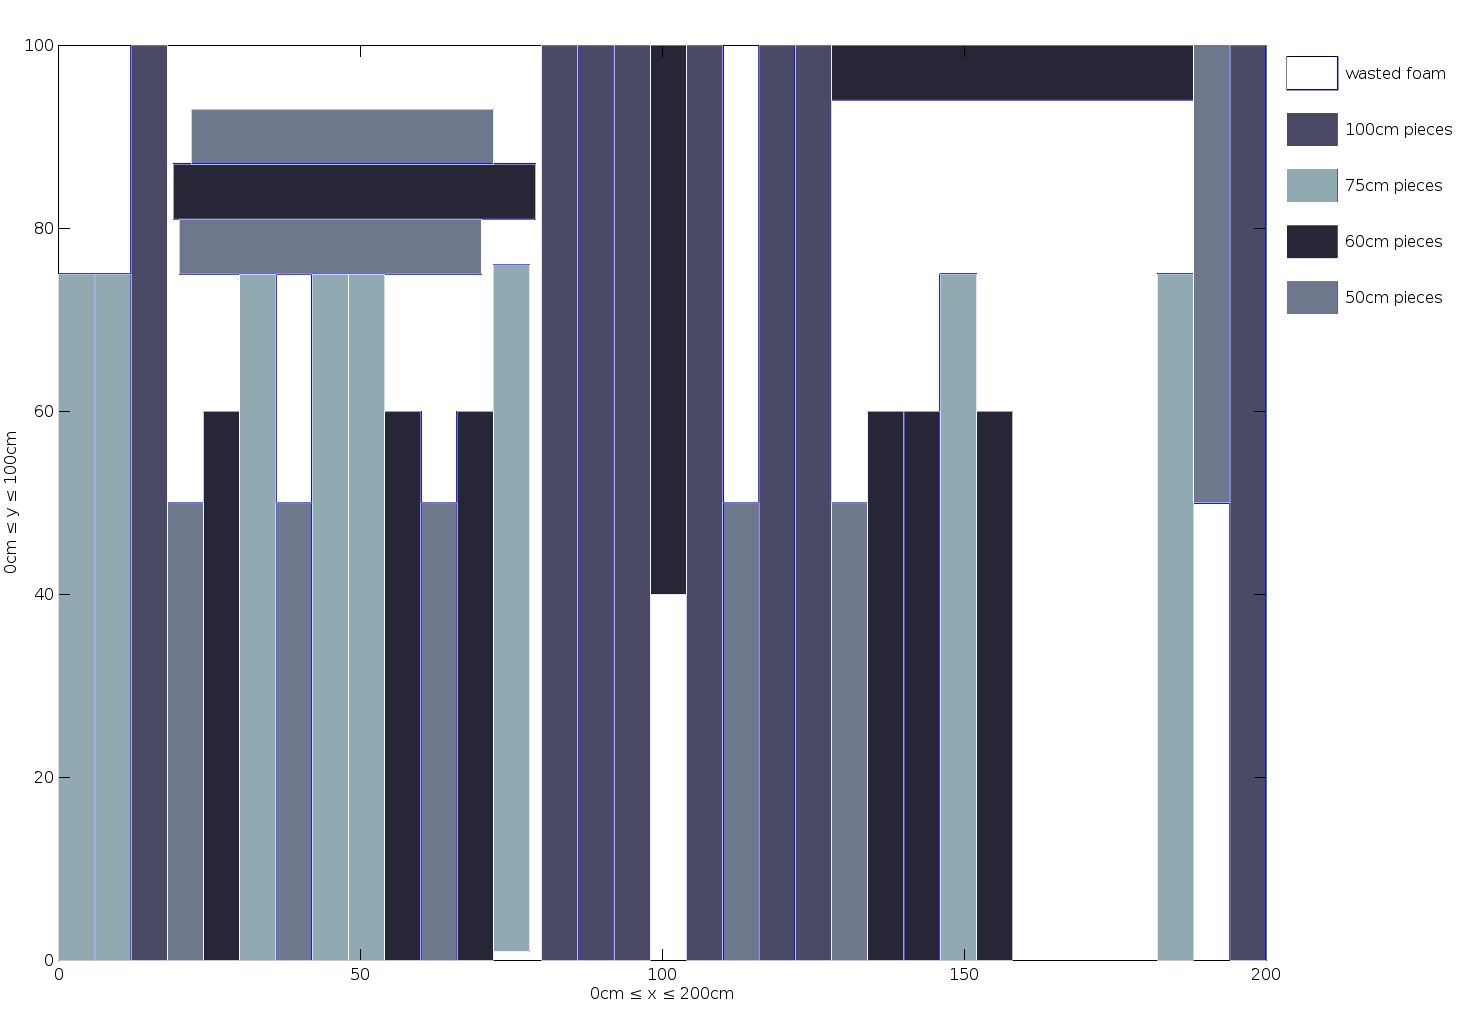
\includegraphics[scale=0.2]{FoamCutting/MIP10mins.png} 
\caption{Solution to the MIP after 10 minutes}
\label{fig:10minsol}
\end{figure}

\begin{figure}
\centering
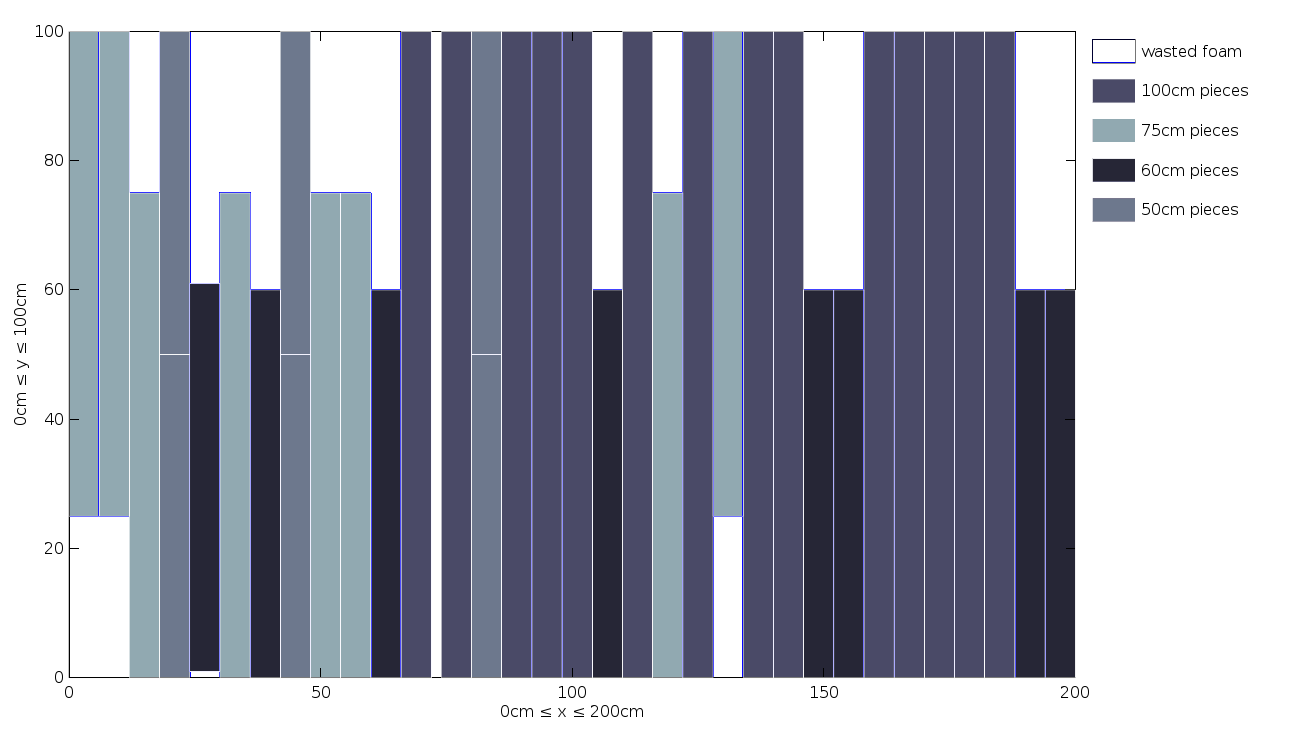
\includegraphics[scale=0.25]{FoamCutting/MIP2hours.png} 
\caption{Solution to the MIP after 2 hours}
\label{fig:12hoursol}
\end{figure}

Even after 12 hours, the solution from the MIP is still not able to match the utility of the solution from the heuristic approach. The difficulties in finding quality solutions within a time limit is not unexpected as the problem is known to be NP-hard. To address this, more complicated heuristics and approximation algorithms could be used as solution approaches in an attempt to reduce the optimality gap. This would be interesting from a mathematical point of view but is of no benefit to the Sports Jugger volunteers who are satisfied with a fast and `good enough' solution. 
% 10 mins 9.76 32.99\%
%  12 hours (IDE) 43200.12s, 10.83 at 19.8\% gap (still 12.98 best bound)


\section{Results and Discussion}
\label{section:results}

Previous methods of constructing equipment did not attempt to use any optimisation at all. Either a different type of foam was used, one that did not come in blocks needing to be cut, or a simple method of cutting the entire block into $1m \times 6cm$ strips was used. These pieces were then consumed whenever individual new items were needed. For comparison purposes, we assume that $1m$ pieces cut from the previous approach would be assigned to items using a greedy method.

The heuristics presented in this paper outperformed the solution obtained from the previous $1m$ strip cutting method. The heuristic solution returned an additional piece of equipment per foam block and converted wastage into pieces suitable for storage. The utility of items completed from a single foam block was increased by 4.5\%. This is shown in Table \ref{tab:compare_results}. 

In these results, we are also able to calculate the relative optimality gap for the exact and heuristic solution approaches by using the best bound found from CPLEX. We find that the heuristic solution has an optimality gap of 10\%. A solution from a heuristic is not guaranteed to be optimal. However, the rules implemented satisfied the requirement for simplicity and that the solution be quick to generate. The pattern was given to the volunteers so that they could cut the foam blocks and begin construction of the needed equipment for the Sports Jugger tournament.


\begin{table}
\begin{tabular}{r|ccccc}
\textit{Item} & Previous & Heuristic & Modified & MIP (10mins) & MIP (12hrs)\\\hline
\textit{Q-tip} &2&\textbf{3}&\textbf{3}&2&2\\
\textit{Staff}  &\textbf{3}&\textbf{3}&\textbf{3}&2&\textbf{3}\\
\textit{Long}&3&3&3&2&\textbf{4}\\
\textit{Short} &5&5&\textbf{6}&4&4\\\hline
\textit{TOTAL} &13&14&\textbf{15}&10&13\\
\textit{Utility1} &11 &11.5 &\textbf{11.75} &9.5& 11\\
\textit{Spare} &&$1\times 100cm$,&$1\times 100cm$,&$1\times 60cm$&\\
\textit{lengths}& &$4 \times 50cm$ &$4 \times 50cm$ &$4 \times 50cm$ & \\
\textit{Utility2} &0&0.3&0.3&0.26&0\\
\textit{Utility3} &11&11.8&12.05&9.76&11\\
\textit{Wastage} & 18.1\% &\textbf{1.9\%} &2.8\% &29.8\%&16.6\%\\\hline
\end{tabular}
\caption{Comparison of resulting equipment obtained from each solution approach. \textit{Utility1} is the utility of completed items. \textit{Utility2} is utility of leftover pieces. \textit{Utility3} is combined utility for all items and pieces. \textit{Wastage} is the amount of foam thrown away due to cutting and trimming.}
\label{tab:compare_results}
\end{table}

% 10 mins 9.76 32.99\%
%  12 hours (IDE) 43200.12s, 10.83 at 19.8\% gap (still 12.98 best bound)
          
%\textbf{need to update this after a new 12 hour run. out of memory at 4000s, (a bit more than an hour) 49.63\% gap and 8.675 solution. not as good as our 15 min solution? What other constraints can we add that are reasonable? warm start? Simply adding, make at least two of each struggles to find the initial feasible solution. Should I be doing a warm start in a main file separate to the mod? seems like a lot of work for this project. Note, I have since found the setting to place node file on disk rather than memory - that should help. Have added more symmetry breaking constraints. Maybe could also add minimum number completed (8 to complete for two teams worth)\\ also got 9.95 in 15 mins?
% optimality gap: best bound from MIP is 12.98. This gives gaps (for our original and heuristic solutions) of 0.18, 0.1 and 0.077. That is 10\% for the first heuristic solution and 7.8\% for the modified heuristic solution.}

An unexpected result of the simplicity of the pattern was that the volunteers were able to manually relax the assumption that pieces will always be cut to the maximum allowable length. The volunteers constructing Sports Jugger equipment made the decision to reduce the size of the Short Spars from $75cm$ of foam padding to $60cm$ of padding after seeing the proposed cutting pattern. This allowed them to modify the cutting pattern and construct one more piece of equipment from the same block of foam. After the foam blocks were cut, we continued work on developing an optimal solution using mathematical programming. 

It was found that it took significant time to improve solutions with exact solution approaches even for a single block of foam. We were able to find solutions within minutes but these were outperformed by the heuristic solution. Solutions after a longer period of time showed improvement but not enough to match heuristic solutions. 

Further work comparing solution approaches could explore a MIP model which includes some of the additional assumptions from the heuristic approaches. That is, requiring guillotine cuts and a minimum number of pieces of the same type to be cut adjacent would reduce the solution space if added into the MIP model as constraints. This would possibly remove some good solutions but would provide more useful solutions in a reasonable amount of time. Alternatively, the heuristic solution could be used as a warm start to an exact solver. Initial attempts at a partial warm start have been promising. but slow down once we reach the minimum partial set.

We also found a good solution through a fortuitous error in the mathematical model. An earlier, incorrect formulation of the mathematical model restricts the placement of pieces to be cut. Pieces overlapping in the $x-$dimension require that the piece with a larger index be positioned above the piece with a smaller index, excluding solutions where the larger indexed piece would fit below the other. Similarly, pieces overlapping in the $y-$ dimension require that that the piece with a larger index be positioned to the right of the piece with a smaller index. This reduces the solution space and potentially excludes the optimal solution. However, we found that solving this model in CPLEX returned very good solutions within a 10 minute time limit even though it also struggled to prove optimality with a longer time limit.

A consequence of this particular error is that pieces of the same type are grouped together because of sequential indices. The resulting solutions therefore contain subsections where multiple pieces of the same type are cut - similar to one of the assumptions in the heuristic solution.  Indeed, the solution returned from this model was similar in appearance to the heuristic solution but outperformed the initial heuristic solution. It returned the exact same number of completed items as the modified heuristic solution but had fewer spare pieces able to be stored. The solution from this approach is shown in Figure \ref{fig:MIPerror}. This cutting pattern remains easy for volunteers to comprehend and implement. Manual adjustments can still be made if necessary, for example the pattern can be shifted to the right by $6cm$. This would remove the $6cm$ section on the right hand side of the block as a section this narrow is unappealing to cut by hand. Instead, the width of the section dedicated to $100cm$ pieces could be increased.

\begin{figure}
\centering
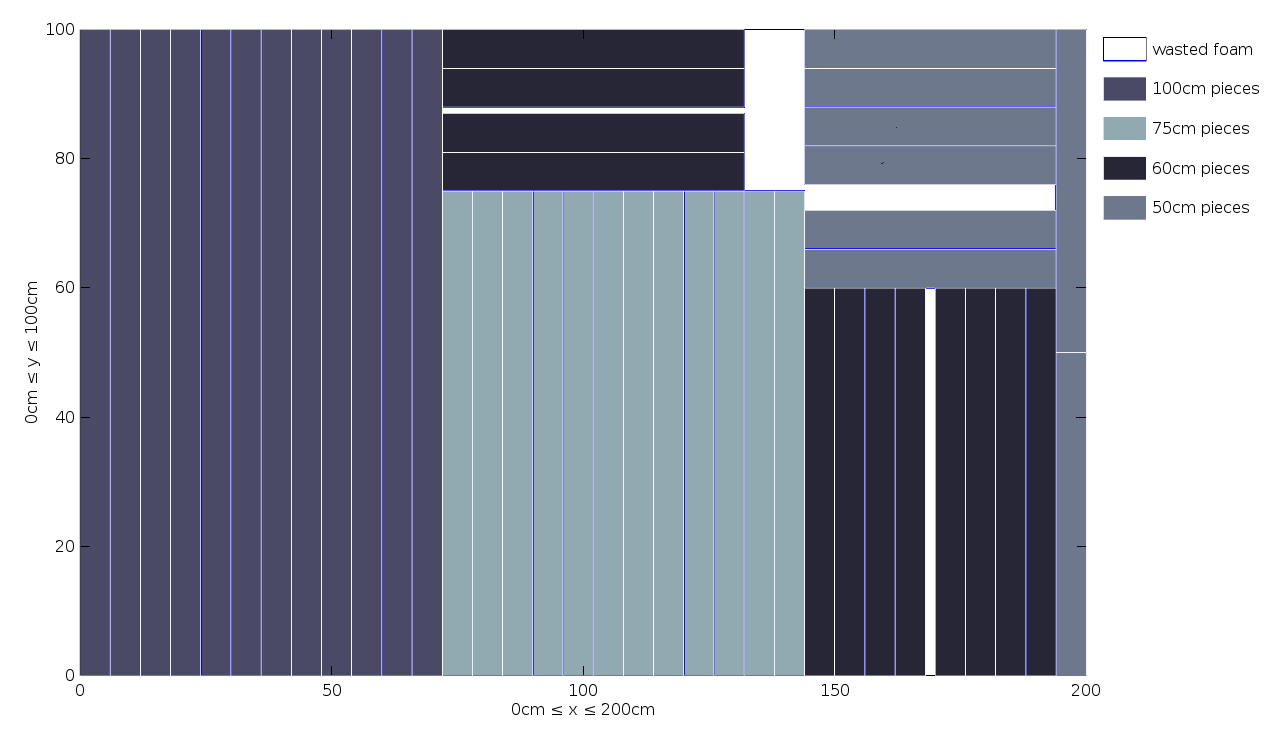
\includegraphics[scale=0.3]{FoamCutting/MIPerrored.png} 
\caption{Solution from a MIP with a reduced solution space and 10 min time limit}
\label{fig:MIPerror}
\end{figure}

Interestingly, the solution obtained from the correct MIP in 12 hours was not able to reach solutions with the utility of the heuristic solution or the incorrect MIP. The correct MIP model would be expected to improve teh solution if given enough time. Furthermore, guillotine cuts could be implemented in the MIP model. This would reduce the solution space in line with realistic assumptions and potentially find quality solutions faster.

The most appropriate solution approach to use for the type of problem considered in this paper will strongly depend on the preferences of those requiring the solution. These preferences may include the simplicity of cutting patterns, storing (or not storing) spare pieces and whether items shorter than the maximum allowable length are acceptable. More importantly, do these preferences lend themselves to assumptions that would reduce the solution space of a MIP model and what resources do the problem owners have for solving a MIP with exact methods?

The best solution found in this paper was a manual modification of a heuristic solution. The heuristic approach returns solutions that have a guaranteed minimum size for each section to be cut and will avoid trimming. Pieces are assigned to items in order of item utility for that specific piece length. The heuristic solution presents appealing cutting patterns, reduces the amount of foam wasted and supplies a number of pieces to be stored for future use. The modified heuristic solution provided a greater quantity of Sports Jugger equipment by making a manual tradeoff with the size of each item of equipment. This manual adjustment was only possible because of the simplicity of the heuristic solution. 

Further work on this topic would extend the solution approaches to consider multiple foam blocks and existing supplies (both spare pieces and complete items in stock). A simple approach to including existing club supplies would be to change the benefit values assigned to each item constructed. The model may also be extended to consider the full cost of constructing Sports Jugger equipment, including the cost of cores as well as foam padding.  

\section{Conclusion}
This paper briefly describes a packing and assignment problem encountered when constructing equipment for Sports Jugger. Part of the expense of constructing equipment is due to necessary foam padding. We introduce a formulation for a 2D knapsack problem to find a good cutting pattern for a single block of foam. This problem also integrates the assignment of cut pieces to items of equipment. We maximise the utility of a single block of foam by determining which pieces should be cut, and either used immediately or stored for later use, and which items to construct from those pieces. 

A heuristic solution approach improved upon the cutting pattern previously used yet retained simplicity. It was well received and implemented by volunteers. We go on to show that a MIP model using disjunctive constraints can also generate a cutting pattern but struggles to match the heuristic solution within a useful amount of time. Additional work on improving solution approaches, or introducing additional constraints, can improve the quality of solutions found by solving a MIP model within a reasonable time limit. However, heuristic solution approaches may also be more accessible to small sporting clubs that may not have the resources to implement optimisation models. It is therefore important to work in close collaboration with the people requiring the solution so that the most suitable solution can be provided.

\paragraph{Acknowledgements}
The author would like to thank the mathematical sciences community at IBM Research, Australia for their encouragement to submit this work for publication and helpful suggestions.\\
It is also important to thank the volunteers of the Melbourne Jugger Club and Australian Jugger League Inc. for the  discussions on this problem.

\bibliographystyle{amsplain}
\bibliography{FoamCutting}

\end{document}

%references
%http://pubsonline.informs.org/doi/pdf/10.1287/opre.13.1.94
%http://link.springer.com/chapter/10.1007%2F0-387-25486-2_5
%http://www.sciencedirect.com/science/article/pii/092552739400045X
%http://www.jstor.org/stable/2583579?seq=1#page_scan_tab_contents
%http://link.springer.com/chapter/10.1007/978-3-540-24777-7_8
%http://www.sciencedirect.com/science/article/pii/S030505480700264X
%http://www.sciencedirect.com/science/article/pii/S0305054810002510

% 10 mins 9.76 32.99\%

%completed = [[1
%             1 0 0 0 0 0 0]
%             [1 1 0 0 0 0 0 0]
%             [1 1 0 0 0 0 0 0]
%             [1 1 1 1 0 0 0 0]];
%cut = [1 1 1 1 1 1 1 1 0 0 0 0 0 0 0 0 1 1 1 1 1 1 1 1 0 0 0 0 0 0 0 0 1 1 1
%         1 1 1 1 1 1 0 0 0 0 0 0 0 1 1 1 1 1 1 1 1];
%assigned = [[0 4 4 0]
%             [0 0 0 8]
%             [8 0 0 0]
%             [0 0 4 0]];
%x = [122 92 116 12 80 86 194 104 0 0 0 0 0 0 0 194 182 48 42 6 146 72 30 0 0
%         1 194 194 0 0 0 0 134 24 152 19 140 66 98 54 128 140 0 0 0 0 0 85
%         60 20 128 36 110 188 18 22];
%rotation = [1 1 1 1 1 1 1 1 1 0 0 0 0 0 0 1 1 1 1 1 1 1 1 1 0 0 1 1 0 0 0 0
%         1 1 1 0 1 1 1 1 0 0 0 0 0 0 0 0 1 0 1 1 1 1 1 0];
%y = [0 0 0 0 0 0 0 0 0 0 0 94 0 0 0 0 0 0 0 0 0 1 0 0 0 0 0 0 0 0 0 0 0 0 0
%         81 0 0 40 0 94 0 75 0 94 94 0 94 0 75 0 0 0 50 0 87];

%6 hours 10.2 gap 27.25
%completed 2,4,3,3
%completed = [[1
%             1 0 0 0 0 0 0]
%             [1 1 1 1 0 0 0 0]
%             [1 1 1 0 0 0 0 0]
%             [1 1 1 0 0 0 0 0]];
%cut = [1 1 1 1 1 1 1 1 1 1 1 1 1 1 0 0 1 1 1 1 1 1 0 0 0 0 0 0 0 0 0 0 1 1 1
%         1 1 1 1 1 1 1 0 0 0 0 0 0 1 1 1 1 1 1 0 0];
%assigned = [[0 8 6 0]
%             [0 0 0 6]
%             [8 0 0 0]
%             [0 0 6 0]];
%x = [92 74 68 48 176 134 140 188 158 80 164 128 182 122 0 0 54 18 24 170 98
%         12 0 0 125 125 125 194 0 0 0 0 110 6 152 36 42 104 146 194 116 62
%         0 0 0 0 0 0 30 0 86 30 86 0 86 44];
%y = [0 0 0 0 0 0 0 0 0 0 0 0 0 0 94 0 0 0 1 0 0 0 1 0 0 0 51 0 0 0 0 0 0 0 0
%         0 0 40 40 0 0 0 0 0 0 0 0 94 0 50 50 50 0 0 0 0];
%         rotation = [1 1 1 1 1 1 1 1 1 1 1 1 1 1 0 1 1 1 1 1 1 1 0 0 0 0 0 1 1 1 0 0
%         1 1 1 1 1 1 1 1 1 1 0 1 1 0 0 0 1 1 1 1 1 1 0 1];
%         
%         next: run 12 hours through command prompt
%         
%12 hours (IDE) 43200.12s, 10.83 at 19.8\% gap (still 12.98 best bound)
%         
%        completed = [[1
%             1 0 0 0 0 0 0]
%             [1 1 1 1 0 0 0 0]
%             [1 1 1 0 0 0 0 0]
%             [1 1 1 1 0 0 0 0]];
%cut = [1 1 1 1 1 1 1 1 1 1 1 1 1 1 0 0 1 1 1 1 1 1 1 1 0 0 0 0 0 0 0 0 1 1 1
%         1 1 1 1 1 0 0 0 0 0 0 0 0 1 1 1 1 1 1 0 0];
%assigned = [[0 8 6 0]
%             [0 0 0 8]
%             [8 0 0 0]
%             [0 0 6 0]];
%x = [92 74 98 66 176 134 158 170 140 86 164 122 182 110 0 0 54 12 48 128 116
%         30 6 0 194 0 125 194 0 0 194 0 104 24 152 60 36 146 188 194 98 36
%         0 0 0 0 0 0 42 18 80 42 80 18 62 0];
%rotation = [1 1 1 1 1 1 1 1 1 1 1 1 1 1 1 0 1 1 1 1 1 1 1 1 1 1 0 1 0 1 1 0
%         1 1 1 1 1 1 1 1 1 1 0 1 0 0 0 0 1 1 1 1 1 1 1 1];
%y = [0 0 0 0 0 0 0 0 0 0 0 0 0 0 0 0 0 0 0 25 0 0 25 25 0 0 94 0 0 0 0 0 0 1
%         0 0 0 0 0 0 0 0 50 0 0 0 0 0 0 50 0 50 50 0 0 0];